\documentclass{../../bredelebeamer}
\usepackage{multirow}
\usepackage{pdfpages}
\usepackage{braket,bigstrut}
\usepackage{palatino}
\usepackage{multicol,bigstrut}
\usepackage{listings}
\usepackage{tikz}
\usepackage{pgfplots}
\pgfplotsset{compat=1.17}
\usepackage{booktabs}
\usepackage{amsmath,amssymb,amsfonts,cancel,physics,siunitx}
\usepackage{ragged2e}
\usetikzlibrary{positioning,shadows,backgrounds,calc}%
\setbeamercolor{footnote mark}{fg=black}
\setbeamercolor{footnote}{fg=black}


\renewcommand{\baselinestretch}{0.9}

% \usepackage[backend=bibtex8,style=authortitle,autocite=footnote]{biblatex}
%\addbibresource{../../references.bib}

% \renewbibmacro*{cite:title}{%
% 	\printtext[bibhyperref]{%
% 		\printfield[citetitle]{labeltitle}%
% 		\setunit{\space}%
% 		\printtext[parens]{\printdate}%
% 	}%
% }

\renewcommand{\figurename}{{\bf Fig.}}
\usefonttheme{serif} % default family is serif

\renewcommand{\baselinestretch}{0.9}

\title[Higgs-Portal DM with VBF at HL-LHC]{Probing Higgs-Portal Dark Matter with VBF Signatures at the HL-LHC}
\subtitle{}
\author[C. Rodríguez]{
	\vspace{2em}\\
	MSc. Cristian Fernando Rodríguez Cruz\inst{1}\\
	\vspace{1em}
}

\institute[Uniandes]{\inst{1} Universidad de los Andes\and
% \inst{2} Pontificia Universidad Católica del Perú 
}
\date{\today}
\lstset{language=C++,
  basicstyle=\ttfamily,
  keywordstyle=\color{blue}\ttfamily,
  stringstyle=\color{red}\ttfamily,
  commentstyle=\color{green}\ttfamily,
  morecomment=[l][\color{magenta}]{\#}
}

\begin{document}
\begin{frame}
    \titlepage
\end{frame}
\begin{frame}{Abstract}
    \justifying
    We investigate current and projected constraints on Higgs-portal dark matter (DM) models, focusing on both scalar and fermionic DM candidates, using vector boson fusion (VBF) production of the Higgs boson at the LHC. By analyzing the parameter space in the plane of DM mass versus the Higgs-DM coupling, we aim to reinterpret existing LHC VBF + MET searches to set bounds on the invisible Higgs decay channels.

    \vfill

    To this end, we perform simulations in MadGraph5\_aMC@NLO under LHC conditions to compute cross sections for VBF Higgs production followed by invisible decays. Experimental efficiencies are estimated through a recast of public analyses targeting the process $pp \to jj + \text{MET}$. We then rescale the integrated luminosity to project the reach of the High-Luminosity LHC (HL-LHC), identifying both currently excluded regions and those potentially probed with 3 ab$^{-1}$. Our results provide updated exclusion contours and projections in the Higgs-portal to DM parameter space.
\end{frame}

\begin{frame}{Outline}
    \tableofcontents
\end{frame}

\section{Introduction}
\begin{frame}{Dark Matter: The Missing Piece}
    \begin{itemize}
        \item Evidence for dark matter from cosmological observations
        \item The need for particle physics models beyond the Standard Model
        \item Higgs-portal as a minimal and well-motivated framework
    \end{itemize}
\end{frame}

\section{Theoretical Framework}
\begin{frame}{Vector Boson Fusion (VBF) Production}
    \begin{minipage}{0.38\textwidth}
        \begin{center}
            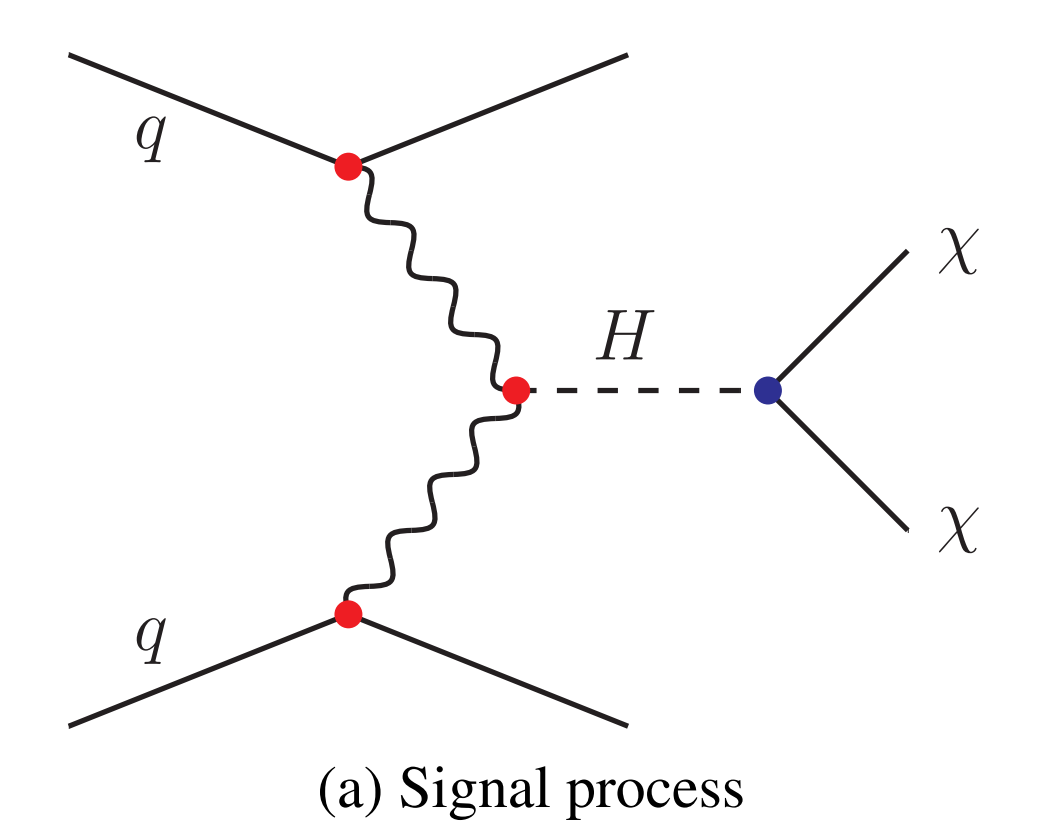
\includegraphics[width=\textwidth]{../Images/VBF.png}
        \end{center}
    \end{minipage}
    \hfill
    \begin{minipage}{0.6\textwidth}
        The Higgs boson is narrow: 
        \begin{equation*}
            \Gamma_h/m_h = 4.07 \text{ MeV}/125 \text{ GeV} \approx 3.3 \times 10^{-5}
        \end{equation*}
        Cross section factorizes into production and decay:
        \begin{multline*}
            \sigma_{\text{total}} = \sigma_{\text{prod}} (\textcolor{red}{pp\boldsymbol{\to}j\,j\, h})  \times \text{BR}(\textcolor{blue}{h \boldsymbol{\to} \text{inv.}})
        \end{multline*}
    \end{minipage}
\end{frame}


\begin{frame}{Higgs-Portal Dark Matter Models}
    \begin{itemize}
        \item Scalar DM candidate: $\mathcal{L} \supset \lambda_s |H|^2 S^2$
        \item Fermionic DM candidate: $\mathcal{L} \supset y_f H \bar{\chi} \chi$
        \item Connection to invisible Higgs decays: $H \to \text{DM} + \text{DM}$
        \item Parameter space: $(m_{\text{DM}}, \lambda/y_f)$
    \end{itemize}
\end{frame}



\begin{frame}{Invisible Higgs Decay Channels}
    \begin{itemize}
        \item $H \to \chi \chi$ (fermionic DM)
        \item $H \to SS$ (scalar DM)
        \item Branching ratios and kinematic constraints
        \item Connection to relic density requirements
    \end{itemize}
\end{frame}

\section{Methodology}
\begin{frame}{Simulation Setup}
    \begin{itemize}
        \item MadGraph5\_aMC@NLO for signal generation
        \item LHC conditions at $\sqrt{s} = 13$ TeV
        \item Process: $pp \to jj + \text{MET}$ via VBF
        \item Systematic uncertainties and scale variations
    \end{itemize}
\end{frame}

\begin{frame}{Experimental Recast}
    \begin{itemize}
        \item Public LHC analyses targeting $pp \to jj + \text{MET}$
        \item Efficiency estimation and acceptance calculations
        \item Background modeling and systematic uncertainties
        \item Statistical treatment of exclusion limits
    \end{itemize}
\end{frame}

\section{Results}
\begin{frame}{Current LHC Constraints}
    \begin{itemize}
        \item Exclusion contours in $(m_{\text{DM}}, \lambda/y_f)$ plane
        \item Comparison between scalar and fermionic DM
        \item Sensitivity to different mass ranges
    \end{itemize}
    % Add plots here
\end{frame}

\begin{frame}{HL-LHC Projections}
    \begin{itemize}
        \item Projected reach with 3 ab$^{-1}$ integrated luminosity
        \item Improvement over current constraints
        \item Complementarity with other search strategies
    \end{itemize}
    % Add projection plots here
\end{frame}

\begin{frame}{Parameter Space Analysis}
    \begin{itemize}
        \item Currently excluded regions
        \item Future sensitivity regions
        \item Comparison with direct detection experiments
        \item Implications for model viability
    \end{itemize}
\end{frame}

\section{Discussion}
\begin{frame}{Theoretical Implications}
    \begin{itemize}
        \item Constraints on Higgs-portal coupling strength
        \item Impact on dark matter relic density
        \item Model-dependent vs. model-independent results
    \end{itemize}
\end{frame}

\begin{frame}{Experimental Considerations}
    \begin{itemize}
        \item Systematic uncertainties and their impact
        \item Comparison with other Higgs production modes
        \item Future improvements and detector upgrades
    \end{itemize}
\end{frame}

\section{Conclusions}
\begin{frame}{Summary}
    \begin{itemize}
        \item VBF provides competitive constraints on Higgs-portal DM
        \item HL-LHC will significantly extend the reach
        \item Both scalar and fermionic DM models constrained
        \item Complementary approach to direct/indirect detection
    \end{itemize}
\end{frame}

\begin{frame}{Future Outlook}
    \begin{itemize}
        \item Extension to other DM models
        \item Combination with other search channels
        \item Implications for future collider experiments
        \item Connection to cosmological observations
    \end{itemize}
\end{frame}

\begin{frame}
    \centering
    \Huge Thank you for your attention!
    \vfill
    \Large Questions?
\end{frame}
\end{document}